\documentclass[dvipdfmx]{beamer}

\usetheme{Boadilla}
\setbeamertemplate{navigation symbols}{}

\usepackage{bxdpx-beamer}
\usepackage{amsmath}
\usepackage{amssymb}
\usepackage{amsfonts}
\usepackage{ascmac}
\usepackage{graphics}
\usepackage{pxjahyper}
\usepackage{hyperref}
\usepackage{listings, jvlisting}
\hypersetup{%
 setpagesize=false,%
 bookmarks=true,%
 bookmarksdepth=tocdepth,%
 bookmarksnumbered=true,%
 colorlinks=true,%
 anchorcolor=black,%
 linkcolor=black,%
 pdftitle={},%
 pdfsubject={},%
 pdfauthor={},%
 }
\lstset{
 basicstyle={\ttfamily},
 identifierstyle={\small},
 commentstyle={\smallitshape},
 keywordstyle={\small\bfseries},
 ndkeywordstyle={\small},
 stringstyle={\small\ttfamily},
 frame={tb},
 breaklines=true,
 columns=[l]{fullflexible},
 numbers=left,
 xrightmargin=0zw,
 xleftmargin=3zw,
 numberstyle={\scriptsize},
 stepnumber=1,
 numbersep=1zw,
 lineskip=-0.5ex,
 showstringspaces=false,
 showtabs=false,
 showspaces=false,
 tabsize=4,
}

%\renewcommand\familydefault{\ttdefault}

\title{演習問題}
\author{Koki Ukeba}
\date{\today}

\begin{document}
\maketitle

\section{はじめに}
\begin{frame}
	\frametitle{はじめに}
	 資料内の演習問題に対する、参考コードはgithub.comのKokiUkebaにあります。動作環境はgcc (Ubuntu 11.4.0-1ubuntu1~22.04) 11.4.0です。
\end{frame}

\begin{frame}[allowframebreaks]
    \tableofcontents
\end{frame}

\section{Lesson1}
\begin{frame}
	\frametitle{プログラミングの基本}
    \framesubtitle{文字列の出力}
	\begin{itembox}[l]{Q1.1}
		"Hello world"という文字列を出力するコードを作成せよ.
	\end{itembox}
	\begin{block}{入力}
	\end{block}
	\begin{block}{出力}
		Hello world.
	\end{block}
\end{frame}

\begin{frame}
    \frametitle{プログラミングの基本}
    \framesubtitle{文字定数}
	\begin{itembox}[l]{Q1.2}
		"$\backslash$"?"を出力するコードを作成せよ。
	\end{itembox}
	\begin{block}{入力}
	\end{block}
	\begin{block}{出力}
        $\backslash$"?
	\end{block}
\end{frame}

\begin{frame}
    \frametitle{プログラミングの基本}
    \framesubtitle{文字定数}
	\begin{itembox}[l]{Q1.3}
        16進数のdeadbabeを10進数で出力してください。
	\end{itembox}
	\begin{block}{入力}
	\end{block}
	\begin{block}{出力}
        -559039810
	\end{block}
\end{frame}

\begin{frame}
    \frametitle{プログラミングの基本}
    \framesubtitle{文字定数}
	\begin{itembox}[l]{Q1.4}
        16進数のdeadbabeを入力し,10進数表示が-559039810であることを確認せよ。
	\end{itembox}
	\begin{block}{入力}
        deadbabe
	\end{block}
	\begin{block}{出力}
        -559039810
	\end{block}
\end{frame}

\begin{frame}
    \frametitle{プログラミングの基本}
    \framesubtitle{文字定数}
	\begin{itembox}[l]{Q1.5}
        10進数の-559039810を入力し,16進数表示がdeadbabeであることを確認せよ。
	\end{itembox}
	\begin{block}{入力}
        -559039810
	\end{block}
	\begin{block}{出力}
        deadbabe
	\end{block}
\end{frame}

\section{Lesson2}
\begin{frame}
	\frametitle{変数~繰り返しを添えて~}
	\begin{itembox}[l]{Q-2}
		ライプニッツ級数
		$$\sum_{n=0}^{\infty}\frac{(-1)^n}{2n+1}$$
		が$\dfrac{\pi}{4}$に収束することを確かめてください。
		また、その計算結果と$\pi$とを比較してください。
	\end{itembox}
	\begin{block}{入力}
	\end{block}
	\begin{block}{出力}
		$\mathsf{calc = 0.7853956634}$\\
		$\mathsf{M\_PI/4 = 0.7853981634}$\\
		$\mathsf{dif = 0.0000025000}$
	\end{block}
\end{frame}

\begin{frame}
    \frametitle{演算}
    \framesubtitle{シフト演算子}
	\begin{itembox}[l]{Q2.1}
        "$<<$"及び"$>>$"はシフト演算子と呼ばれ,
        $$x <<(>>) n$$
        はxを左(右)へn[bit]シフトさせることを意味する。\\
        この演算子を利用し、入力した整数値$a$の$2^b$倍の値を出力するコードを作成せよ。
	\end{itembox}
	\begin{block}{入力}
        1\\
        5
	\end{block}
	\begin{block}{出力}
        32
	\end{block}
\end{frame}

\begin{frame}
    \frametitle{演算}
    \framesubtitle{モジュロ演算子, 否定演算子}
	\begin{itembox}[l]{Q2.2}
        "\%"はモジュロ演算子と呼ばれ、
        $$x \% y$$
        はxをyで割ったときのあまりとなる。\\
        "!"は否定演算子と呼ばれ、
        $$!x$$
        はxが0のときのみ1となる。\\
        この演算子を利用し、入力した整数値aがbを因数に持つときのみbを出力し、bを因数に持たない場合は0を出力するコードを作成せよ。
	\end{itembox}
    \vspace{-30pt}
    \begin{columns}[t, totalwidth=0.98\linewidth]
        \begin{column}{.45\linewidth}
            \begin{block}{入力}
                1001\\
                11
            \end{block}
        \end{column}
        \begin{column}{.45\linewidth}
            \begin{block}{出力}
                11
            \end{block}
        \end{column}
    \end{columns}
\end{frame}

\begin{frame}
    \frametitle{演算}
    \framesubtitle{3項演算子}
	\begin{itembox}[l]{Q2.3}
        "? :"は3項演算子と呼ばれ,ある式を$expr_{i}(i=1,2,3)$とすると、
        $$expr_{1} ? expr_{2}:expr_{3}$$
        は$expr_{1}$が0ではない場合(真の場合)$expr_{2}$の値となり、そうでない場合は$expr_{3}$の値となる。\\
        この演算子を利用し、整数値aの絶対値を出力するコードを作成せよ。
	\end{itembox}
	\begin{block}{入力}
        -18
	\end{block}
	\begin{block}{出力}
        18
	\end{block}
\end{frame}

\begin{frame}
    \frametitle{演算}
    \framesubtitle{ASCII}
	\begin{itembox}[l]{Q2.4}
        ASCII文字セットのある1文字(半角英語)を入力した際に,その文字の大文字小文字を変換するコードを作成せよ。半角英語以外の値が入力されたときの処理は自由にしてよい。
	\end{itembox}
	\begin{block}{入力}
        A
	\end{block}
	\begin{block}{出力}
        a
	\end{block}
\end{frame}

\begin{frame}
    \frametitle{演算}
    \framesubtitle{変数の型}
	\begin{itembox}[l]{Q2.5}
        浮動小数点型の数を入力し、その数の整数部と小数部を分けて表示するコードを作成せよ。
	\end{itembox}
	\begin{block}{入力}
        3.141592
	\end{block}
	\begin{block}{出力}
        3, 0.141592
	\end{block}
\end{frame}

\section{Lesson3}
\begin{frame}
	\frametitle{条件分岐}
	\begin{itembox}[l]{Q3.1}
		実数a,b,cが任意に与えられた際に、二次方程式
		$$ax^2+bx+c=0$$
		の解を表示するコードを作成してください。(a=0のときの処理は自由にしてください。)
	\end{itembox}
	\begin{block}{入力}
    1\\
    2\\
    1
	\end{block}
	\begin{block}{出力}
		$\mathsf{1.0x^2 + 2.0x + 1.0 = 0}$\\
		$\mathsf{double \ root -1.0e+00}$
	\end{block}
\end{frame}

\begin{frame}
	\frametitle{条件分岐}
	\begin{block}{出力例2}
		$\mathsf{1.0x^2 + 1.0x + 2.0 = 0}$\\
		$\mathsf{-5.0e-01 + I * 1.3e+00, -5.0e-01 - I * 1.3e+00}$
	\end{block}
	\begin{block}{出力例3}
	$\mathsf{0.0x^2 + 2.0x + 1.0 = 0}$\\
	$\mathsf{single \ root -5.0e-01}$
	\end{block}
	\begin{block}{出力例4}
		$\mathsf{0.0x^2 + 0.0x + 1.0 = 0}$\\
		$\mathsf{no\ solution}$
	\end{block}
\end{frame}

\section{Lesson4}
\begin{frame}
    \frametitle{反復}
    \framesubtitle{for文}
	\begin{itembox}[l]{Q4.1}
        任意の整数値を入力し、その2進数表記を出力するコードを作成せよ。
	\end{itembox}
	\begin{block}{入力}
        70241
	\end{block}
	\begin{block}{出力}
        00000000000000010001001001100001
	\end{block}
\end{frame}

\begin{frame}
    \frametitle{反復}
    \framesubtitle{while文}
	\begin{itembox}[l]{Q4.2}
        任意の正の整数値を入力したとき、その数が素数の場合は1を出力し、素数でない場合は0を出力するコードを作成せよ。
	\end{itembox}
	\begin{block}{入力}
        13
	\end{block}
	\begin{block}{出力}
        1
	\end{block}
\end{frame}

\begin{frame}
    \frametitle{反復}
    \framesubtitle{素数判定}
	\begin{itembox}[l]{Q4.3}
        1~10000000の間にある素数を全て出力するコードを作成せよ。\\
        ただし実行時間が1分を超えるものは不正解とする。
	\end{itembox}
	\begin{block}{入力}
	\end{block}
	\begin{block}{出力}
        (略)
	\end{block}
\end{frame}

\begin{frame}
	\frametitle{Newton-method}
	\begin{itembox}[l]{Q-4}
		ニュートン法を用いて
		$$f(x) = x^3-2x^2-3x+3$$
		の近似解を求めて下さい。\\
		(初期値を1とし、誤差の許容値$\delta$は$10^{-7}$としてください。)\\
		($f'(x)$は自分で求めて大丈夫です。)\\
		(ニュートン法の簡単な説明は次ページにありますが、詳しい解説は各自で調べてください。)
	\end{itembox}
	\begin{block}{入力}		
	\end{block}
	\begin{block}{出力}
		7.608767e-01
	\end{block}
\end{frame}

\begin{frame}
	%\frametitle{Newton-method}
	\begin{itembox}[l]{ニュートン法}
		\begin{enumerate}
			\item 初期値$x_a$を求めたい解になるべく近い値にとる。
			\item もし$\left\lvert f(x_a) \right\lvert \leq \delta $の場合はこの$x_a$を近似解とする。
			\item 上の条件が成り立たない場合は次の代入式により$x_a$を更新して2.へ戻る。
				$$x_a = x_a - \frac{f(x_a)}{f'(x_a)}$$
		\end{enumerate}
	\end{itembox}
	\begin{figure}[h]
		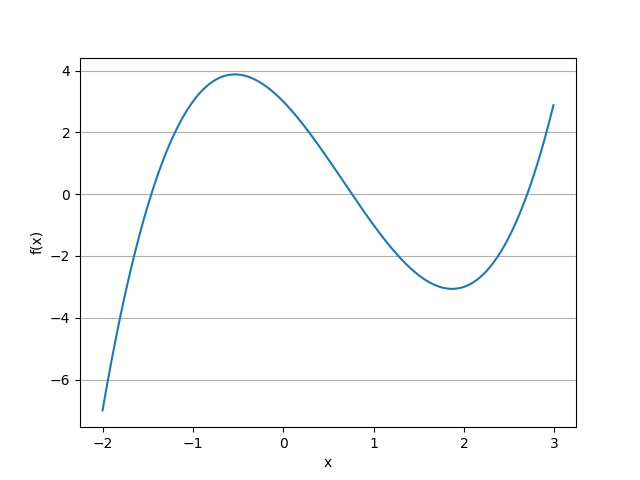
\includegraphics[width=65mm]{Figure_1.png}
	\end{figure}
\end{frame}

\section{Lesson5}
\begin{frame}
	\frametitle{素因数分解}
	\begin{itembox}[l]{Q-5}
		変数に2以上の値を代入し、その数を素因数分解して得られる素数をすべて表示してください。\\
		最終的に変数に119028, 2146654199の2数を代入し出力してください。
	\end{itembox}
	\begin{block}{入力}
	\end{block}
	\begin{block}{出力例1}
		429 =\\
		3 ** 1\\
		11 ** 1\\
		13 ** 1\\
		49238 =\\
		2 ** 1\\
		7 ** 1\\
		3517 ** 1
	\end{block}
\end{frame}

\begin{frame}
	\begin{block}{出力例2}
		7502751 =\\
		3 ** 2\\
		47 ** 1\\
		17737 ** 1\\
		5104981 =\\
		7 ** 1\\
		17 ** 1\\
		42899 ** 1\\
	\end{block}
	\begin{block}{出力例3}
		9562 =\\
		2 ** 1\\
		7 ** 1\\
		683 ** 1\\
		515 =\\
		5 ** 1\\
		103 ** 1
	\end{block}
\end{frame}

\section{Lesson6}
\begin{frame}
	\frametitle{ベクトルの内積}
	\begin{itembox}[l]{Q-6}
		大きさNのdouble型の配列a,bは、すべての要素に値が入った状態で与えられているとします。\\
		$$a = (1,2,3,\dots,N)$$
		$$b = (N, N-1, N-2,\dots,1)$$
		さらに、$N=1001$とし、その内積となす角を求めよ。
	\end{itembox}
\end{frame}

\section{ソートアルゴリズム}
\begin{frame}[t, fragile]
    \frametitle{ソートアルゴリズム}
    \framesubtitle{バブルソート(bubble sort)}
    \begin{itembox}[l]{Q7.1}
        バブルソートとは、隣り合う要素の大小を比較しながら整列させるアルゴリズムである。これをCで実装せよ。下にPythonで実装したコードの一部を示した.
    \end{itembox}
    \begin{lstlisting}[gobble=8, caption=bubbleSort.py, label=bubbleSort]
        data = []

        for i in range(20):
            data.append(randint(0, 100))

        for i in data:
            for j in range(len(data)-1, 0, -1):
                if (data[j] < data[j-1]):
                    data[j], data[j-1] = data[j-1], data[j]
    \end{lstlisting}
\end{frame}

\begin{frame}[t, fragile]
    \frametitle{ソートアルゴリズム}
    \framesubtitle{選択ソート(selection sort)}
    \begin{itembox}[l]{Q7.2}
        選択ソートとは,要素の最大値または最小値を探索し並び変えるアルゴリズムである。これをCで実装せよ。
    \end{itembox}
    \begin{lstlisting}[gobble=8, caption=selectionSort.py, label=selectionSort]
        data = []

        for i in range(len(data)):
            mini = i

            for j in range(i + 1, len(data)):
                if (data[j] < data[mini]):
                    mini = j

            if (mini != i):
                data[i], data[mini] = data[mini], data[i]
    \end{lstlisting}
\end{frame}

\begin{frame}[t, fragile, allowframebreaks]
    \frametitle{ソートアルゴリズム}
    \framesubtitle{カウントソート(counting sort)}
    \begin{itembox}[l]{Q7.3}
        これをCで実装せよ。
    \end{itembox}
    \begin{lstlisting}[gobble=8, caption=countingSort.py, label=countingSort]
        data = []
        dmin = 0
        dmax = 100
        N = 100

        for i in range(N):
            data.append(random.randint(dmin, dmax))

        mini = data[0]
        maxi = data[0]

        for i in range(len(data)):
            if (data[i] < mini):
                mini = data[i]
            if (data[i] > maxi):
                maxi = data[i]

        countLen = maxi - mini + 1
        count = []

        for i in range(countLen):
            count.append(0)

        for i in range(len(data)):
            count[data[i] - mini] += 1

        index = 0
        i = 0
        while (index < len(data)):
            if (count[i] != 0):
                data[index] = i
                index += 1
                count[i] -= 1
            else:
                i += 1
    \end{lstlisting}
\end{frame}

\begin{frame}[t, fragile]
    \frametitle{ソートアルゴリズム}
    \framesubtitle{マージソート(merge sort)}
    \begin{itembox}[l]{Q7.4}
        これをCで実装せよ。
    \end{itembox}
    \begin{lstlisting}[gobble=8, caption=mergeSort.py, label=mergeSort]
        data = []

        for i in range(len(data)):
            mini = i

            for j in range(i + 1, len(data)):
                if (data[j] < data[mini]):
                    mini = j

            if (mini !=  i):
                data[i], data[mini] = data[mini], data[i]
    \end{lstlisting}
\end{frame}

\begin{frame}[t, fragile]
    \frametitle{ソートアルゴリズム}
    \framesubtitle{クイックソート(quiq sort)}
    \begin{itembox}[l]{Q7.5}
        これをCで実装せよ。
    \end{itembox}
    \begin{lstlisting}[gobble=8, caption=mergeSort.py, label=mergeSort]
        data = []

        for i in range(len(data)):
            mini = i

            for j in range(i + 1, len(data)):
                if (data[j] < data[mini]):
                    mini = j

            if (mini !=  i):
                data[i], data[mini] = data[mini], data[i]
    \end{lstlisting}
\end{frame}

\begin{frame}[t, fragile]
    \frametitle{ソートアルゴリズム}
    \framesubtitle{ヒープソート (heap sort)}
    \begin{itembox}[l]{Q7.6}
        これをCで実装せよ。
    \end{itembox}
    \begin{lstlisting}[gobble=8, caption=mergeSort.py, label=mergeSort]
        data = []

        for i in range(len(data)):
            mini = i

            for j in range(i + 1, len(data)):
                if (data[j] < data[mini]):
                    mini = j

            if (mini !=  i):
                data[i], data[mini] = data[mini], data[i]
    \end{lstlisting}
\end{frame}
\end{document}
